\section{Stauanlagen bei Laufwasserkraftwerken}


\subsubsection{Unterschied zu Speicherkraftwerken}
Das Wasser muss immer fliessen können – es kann weder gestoppt noch umgeleitet werden.

\subsubsection{Abfluss}
Muss auch während Instandhaltungsarbeiten gewährleistet sein. Eine mindestens (n-1) -Sicherheit muss für wehrabschlüsse vorhanden sein.
Auch beim Ausfall eines Ablassorgans (Verstopfung) muss das definierte Hächsthochwasser beherrschbar sein.

\subsection{Ausleitungskraftwerke (Umleitungskraftwerke)}

\vspace{0.15cm}

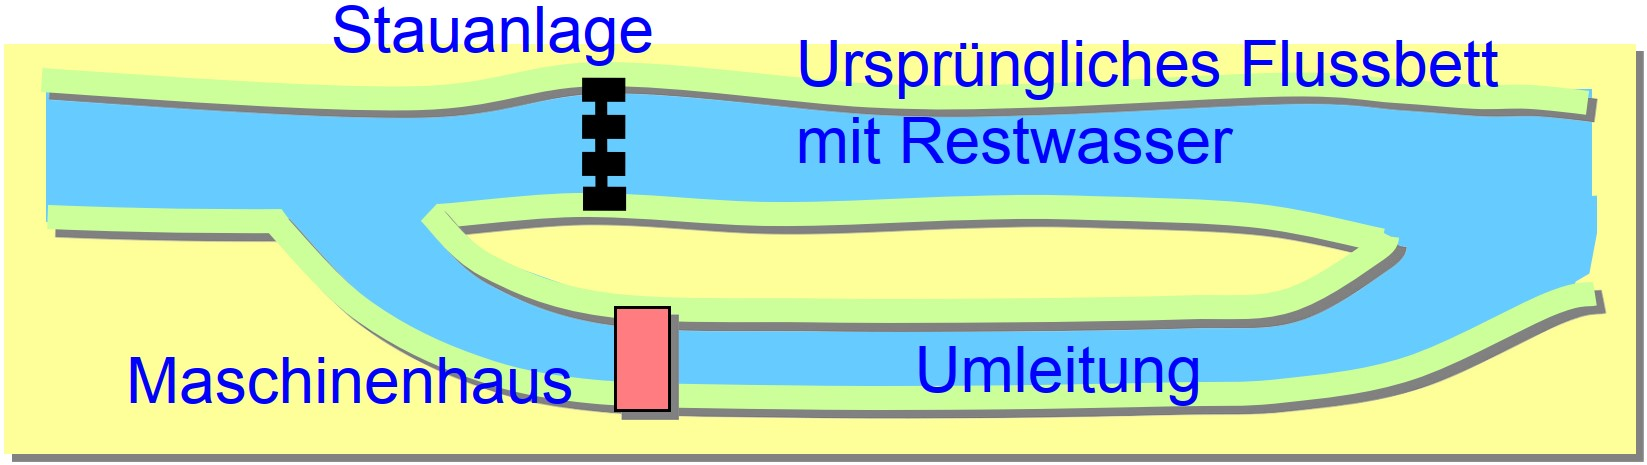
\includegraphics[width=0.98\columnwidth, align=c]{images/Ausleitungskraftwerke.jpg}
\begin{itemize}
  \item Bessere Ausnutzung des Gefälles in flachen Tälern
  \item Wasserwirtschaftliche Belange
  \item Aspekte hinsichtlich des Grundwassers sowie kulturtechnische Erwägungen
  \item Einfacher zum Bauen
\end{itemize}



\subsection{Flusskraftwerke}

\textbf{Bauweise 1}\\
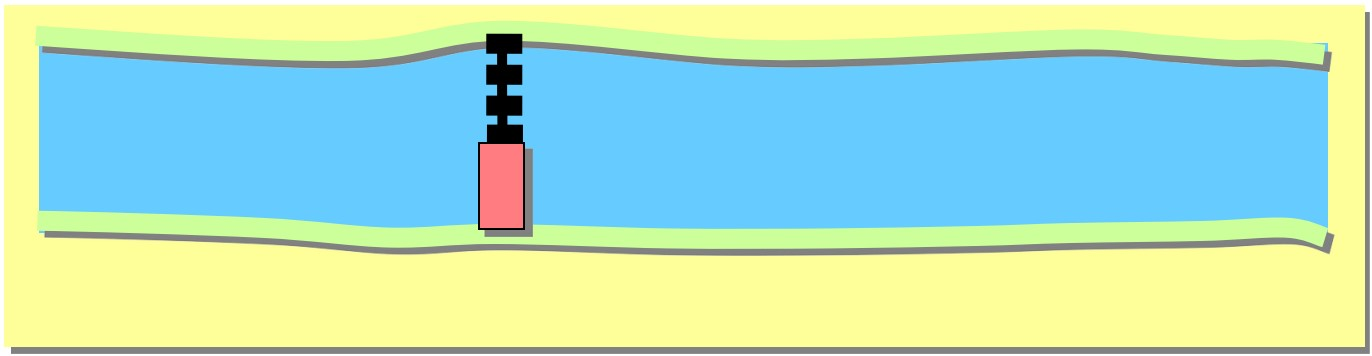
\includegraphics[width=0.98\columnwidth, align=c]{images/Flusskraftwerke_Bauweise_1.jpg}
\vspace{0.15cm}
\textbf{Bauweise 2}\\
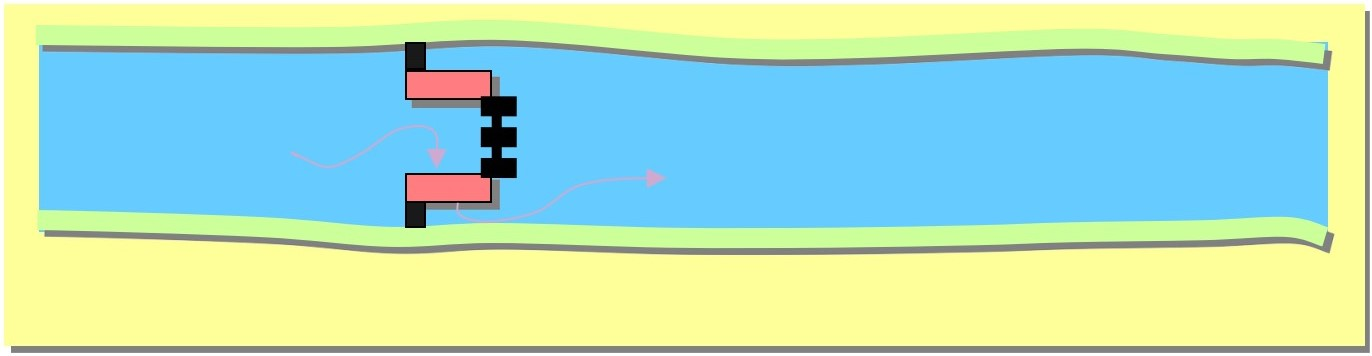
\includegraphics[width=0.98\columnwidth, align=c]{images/Flusskraftwerke_Bauweise_2.jpg}
\vspace{0.15cm}
\textbf{Bauweise 3}\\
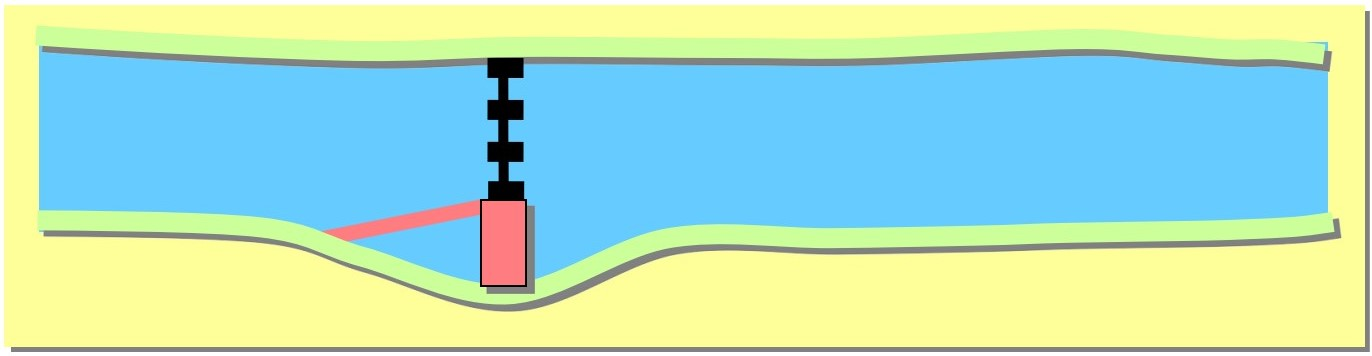
\includegraphics[width=0.98\columnwidth, align=c]{images/Flusskraftwerke_Bauweise_3.jpg}
\vspace{0.15cm}

Moderne Flusskraftwerke werden heute gemäss Bauweise 1 gebaut.

Der Wirkungsgrad bei Bauweise 2 und 3 ist schlechter als bei Bauweise 1.


\subsection{Arten von Wehr- und Sektorverschlüssen}
\includegraphics[width=0.98\columnwidth, align=c]{images/Arten_Wehr_und_Sektorverschlüsse_1.png}

\includegraphics[width=0.98\columnwidth]{images/Arten_Wehr_und_Sektorverschlüsse_2.png}



\subsection{Ort des Maschinenhauses}
Maschinenhaus auf der Kurvenaussenseite

\textbf{\textcolor{green}{Vorteile:}}  
\begin{itemize}
    \item Druckhöhe vor den Trubinen ist grösser
\end{itemize}

\textbf{\textcolor{red}{Nachteile:}}  

\begin{itemize}
    \item Geschwemsel lagert sich vor allem vor dem Rechen ab
    \item Bei starkem Geschwemseltrieb muss eventuell sogar das Kraftwerk abgestellt werden
\end{itemize}

